\documentclass[11pt,fleqn]{article}

\setlength {\topmargin} {-.15in}
\setlength {\textheight} {8.6in}

\usepackage{amsmath}
\usepackage{amssymb}
\usepackage{color}
\usepackage{tikz}
\usetikzlibrary{automata,positioning,arrows}
\usepackage{diagbox}
\usepackage{stackrel}
\begin{document}
Exercise 1.4.12. Write a program that, given two sorted arrays of N int values, prints all elements
that appear in both arrays, in sorted order. The running time of your program
should be $proportional$ to $N$ in the $worst \thickspace case$.\\

Solution

\begin{center}
	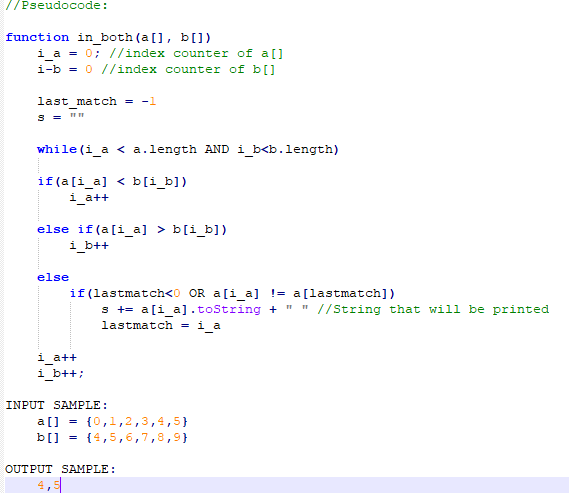
\includegraphics[scale = 1]{1.4.12.png}
	\end{center}


\end{document}

